\section{Model-Based Statistical Analysis} \label{sec:confirmatory}

\subsection{Model Selection}
LRT \cite{wu2009mixed}

\begin{table}[H]
\centering
\begin{tabular}{|l|l|l|}
\hline
& month & month + gender + education \\
\hline
month + gender & 0 & 0.016 \\
\hline
month + education & 0.004 & 0 \\
\hline
\end{tabular}
\caption{P values of Likelihood Ratio tests between models with different covariates under the intervention group}
\label{tab:model.comp.treatment.lrt}
\end{table}

\begin{figure}[H]
\begin{subfigure}{.33\textwidth}
  \centering
  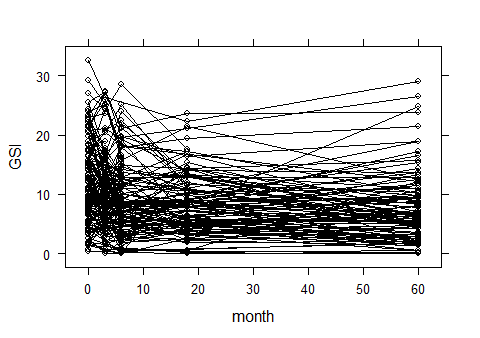
\includegraphics[width=1\linewidth]{../../plots/trellis_treatment.png}
  \caption{trellis plot of all subjects in the intervention group}
\end{subfigure}
\begin{subfigure}{.33\textwidth}
  \centering
  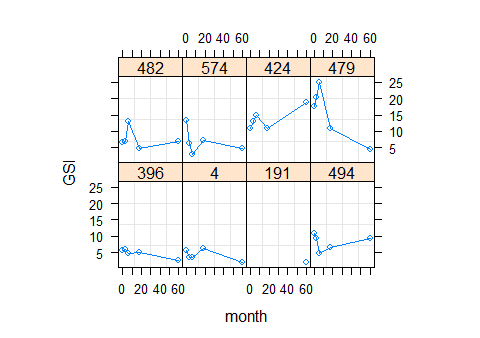
\includegraphics[width=1\linewidth]{../../plots/trellis_subset_treatment.png}
  \caption{trellis plot of randomly selected subjects}
\end{subfigure}
\begin{subfigure}{.33\textwidth}
  \centering
  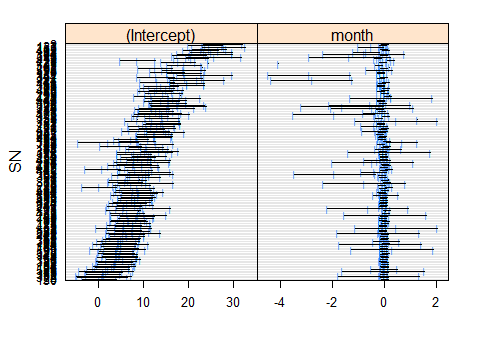
\includegraphics[width=1\linewidth]{../../plots/interval_treatment.png}
  \caption{confidence intervals of parameters from individual linear models}
\end{subfigure}
\caption{Diagnostic plots for selection of random effects for the intervention group}
\label{fig:diagnostic.treatment}
\end{figure}

\begin{table}[H]
\centering
\begin{tabular}{|l|l|l|l|}
\hline
& no mixed effect & intercept & intercept + month \\
\hline
intercept & 0 &/ &/ \\
\hline
intercept + month &/ & 0.028 &/ \\
\hline
intercept + gender &/ & 0.784 &/ \\
\hline
intercept + education &/ & 0.998 &/ \\
\hline
intercept + month + gender & /&/ & 0.893 \\
\hline
intercept + month + education & /&/ & 0.995 \\
\hline
\end{tabular}
\caption{P values of Likelihood Ratio tests between models with different mixed effects under the intervention group}
\label{tab:model.comp.treatment.me.lrt}
\end{table}
\subsection{Assumption Check}

\begin{figure}[H]
\begin{subfigure}{.5\textwidth}
  \centering
  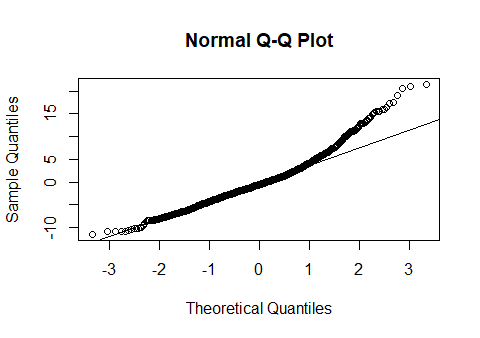
\includegraphics[width=1\linewidth]{../../plots/qq_residual_treatment.png}
  \caption{residual QQ plot}
\end{subfigure}
\begin{subfigure}{.5\textwidth}
  \centering
  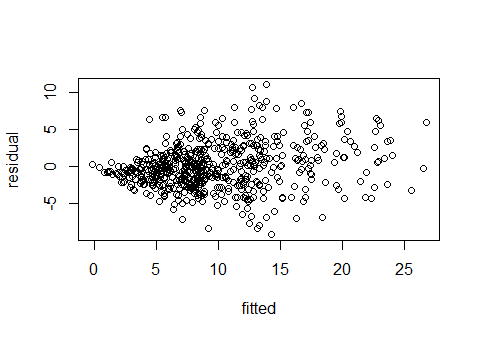
\includegraphics[width=1\linewidth]{../../plots/residual_treatment.png}
  \caption{fitted value vs. residual (t-test: 1, Wilcoxon: 0.204)}
\end{subfigure}
\caption{Visualizing the residuals of the LME model under the intervention group}
\label{fig:residual.treatment}
\end{figure}

\begin{figure}[H]
\begin{subfigure}{.5\textwidth}
  \centering
  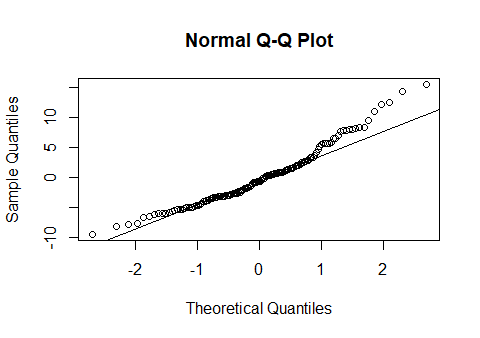
\includegraphics[width=1\linewidth]{../../plots/qq_intercept_treatment.png}
  \caption{QQ plot for the random effects on the intercept (t-test: 1, Wilcoxon: 0.335)}
\end{subfigure}
\begin{subfigure}{.5\textwidth}
  \centering
  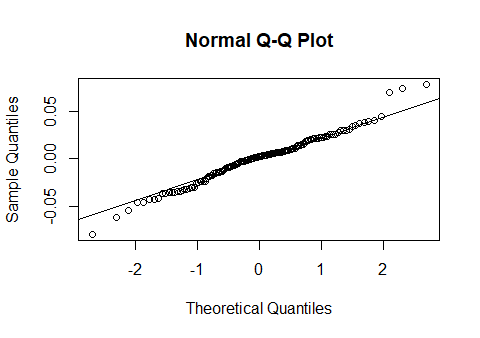
\includegraphics[width=1\linewidth]{../../plots/qq_slope_treatment.png}
  \caption{QQ plot for the random effects on the slope (t-test: 1, Wilcoxon: 0.781)}
\end{subfigure}
\caption{Visualizing the random effects under the intervention group}
\label{fig:re.treatment}
\end{figure}

\subsection{Analysis results}
\subsubsection{Changes in Mental Distress over Time}
\begin{table}[H]
\begin{minipage}{0.5\textwidth}
\centering
\resizebox{\linewidth}{!}{
\begin{tabular}{|l|r|r|r|r|r|}
\hline
  & Value & Std.Error & DF & t-value & p-value\\
\hline
(Intercept) & 11.933 & 2.758 & 465 & 4.326 & 0.000\\
\hline
month & -0.047 & 0.008 & 465 & -5.671 & 0.000\\
\hline
gender2 & 2.764 & 0.925 & 141 & 2.990 & 0.003\\
\hline
education & -0.249 & 0.190 & 141 & -1.314 & 0.191\\
\hline
\end{tabular}
}
\caption{Output of Linear Mixed Model under the intervention group}
\label{tab:lme.treatment}
\end{minipage}
\hfill
\begin{minipage}{0.5\textwidth}
\centering
\resizebox{\linewidth}{!}{
\begin{tabular}{|l|r|r|r|r|r|}
\hline
  & Estimate & Naive S.E. & Naive z & Robust S.E. & Robust z\\
\hline
(Intercept) & 11.162 & 2.484 & 4.494 & 2.538 & 4.397\\
\hline
month & -0.047 & 0.010 & -4.477 & 0.008 & -5.852\\
\hline
gender2 & 2.827 & 0.834 & 3.391 & 0.869 & 3.253\\
\hline
education & -0.194 & 0.170 & -1.146 & 0.173 & -1.125\\
\hline
\end{tabular}
}
\caption{Output of GEE model under the intervention group}
\label{tab:gee.treatment}
\end{minipage}
\end{table}

\begin{table}[H]
\begin{minipage}{0.5\textwidth}
\centering
\resizebox{\linewidth}{!}{
\begin{tabular}{|l|r|r|r|r|r|}
\hline
  & Value & Std.Error & DF & t-value & p-value\\
\hline
(Intercept) & 19.235 & 4.151 & 308 & 4.634 & 0.000\\
\hline
month & -0.020 & 0.008 & 308 & -2.394 & 0.017\\
\hline
gender2 & 2.606 & 1.383 & 95 & 1.884 & 0.063\\
\hline
education & -0.822 & 0.273 & 95 & -3.015 & 0.003\\
\hline
\end{tabular}
}
\caption{Output of Linear Mixed Model under the control group}
\label{tab:lme.control}
\end{minipage}
\hfill
\begin{minipage}{0.5\textwidth}
\centering
\resizebox{\linewidth}{!}{
\begin{tabular}{|l|r|r|r|r|r|}
\hline
  & Estimate & Naive S.E. & Naive z & Robust S.E. & Robust z\\
\hline
(Intercept) & 19.267 & 3.433 & 5.613 & 3.229 & 5.967\\
\hline
month & -0.027 & 0.013 & -2.019 & 0.010 & -2.606\\
\hline
gender2 & 2.220 & 1.148 & 1.935 & 1.216 & 1.825\\
\hline
education & -0.809 & 0.225 & -3.596 & 0.203 & -3.994\\
\hline
\end{tabular}
}
\caption{Output of GEE model under the control group}
\label{tab:gee.control}
\end{minipage}
\end{table}

\subsubsection{Effectiveness of Mental Health Intervention}

\begin{table}[H]
\begin{minipage}{0.5\textwidth}
\centering
\resizebox{\linewidth}{!}{
\begin{tabular}{|l|r|r|r|r|r|}
\hline
  & Value & Std.Error & DF & t-value & p-value\\
\hline
(Intercept) & 15.418 & 2.341 & 774 & 6.586 & 0.000\\
\hline
treatment2 & -0.193 & 0.731 & 238 & -0.264 & 0.792\\
\hline
month & -0.037 & 0.006 & 774 & -5.893 & 0.000\\
\hline
gender2 & 2.737 & 0.776 & 238 & 3.527 & 0.001\\
\hline
education & -0.516 & 0.157 & 238 & -3.295 & 0.001\\
\hline
\end{tabular}
}
\caption{Output of Linear Mixed Model}
\label{tab:lme}
\end{minipage}
\hfill
\begin{minipage}{0.5\textwidth}
\centering
\resizebox{\linewidth}{!}{
\begin{tabular}{|l|r|r|r|r|r|}
\hline
  & Estimate & Naive S.E. & Naive z & Robust S.E. & Robust z\\
\hline
(Intercept) & 14.685 & 2.046 & 7.176 & 2.053 & 7.154\\
\hline
treatment2 & -0.430 & 0.641 & -0.671 & 0.735 & -0.586\\
\hline
month & -0.039 & 0.008 & -4.666 & 0.006 & -6.040\\
\hline
gender2 & 2.693 & 0.680 & 3.961 & 0.716 & 3.763\\
\hline
education & -0.455 & 0.136 & -3.337 & 0.139 & -3.278\\
\hline
\end{tabular}
}
\caption{Output of GEE model}
\label{tab:gee}
\end{minipage}
\end{table}

\subsection{Handling Missing Data}
\cite{little2019statistical}